%%%%%%%%%%%%%%%%%%%% book.tex %%%%%%%%%%%%%%%%%%%%%%%%%%%%%
%
% sample root file for the chapters of your "monograph"
%
% Use this file as a template for your own input.
%
%%%%%%%%%%%%%%%% Springer-Verlag %%%%%%%%%%%%%%%%%%%%%%%%%%


% RECOMMENDED %%%%%%%%%%%%%%%%%%%%%%%%%%%%%%%%%%%%%%%%%%%%%%%%%%%
\documentclass[graybox,envcountchap,sectrefs]{svmono}

% choose options for [] as required from the list
% in the Reference Guide

\usepackage{mathptmx}
\usepackage{helvet}
\usepackage{courier}
%
\usepackage{type1cm}         

\usepackage{makeidx}         % allows index generation
\usepackage{graphicx}        % standard LaTeX graphics tool
                             % when including figure files
\usepackage{multicol}        % used for the two-column index
\usepackage[bottom]{footmisc}% places footnotes at page bottom

% see the list of further useful packages
% in the Reference Guide

\makeindex             % used for the subject index
                       % please use the style svind.ist with
                       % your makeindex program

%%%%%%%%%%%%%%%%%%%%%%%%%%%%%%%%%%%%%%%%%%%%%%%%%%%%%%%%%%%%%%%%%%%%%

\begin{document}

\author{Author name(s)}
\title{Book title}
\subtitle{-- Monograph --}
\maketitle

\frontmatter%%%%%%%%%%%%%%%%%%%%%%%%%%%%%%%%%%%%%%%%%%%%%%%%%%%%%%

%%%%%%%%%%%%%%%%%%%%%%% dedic.tex %%%%%%%%%%%%%%%%%%%%%%%%%%
%
% sample dedication
%
% Use this file as a template for your own input.
%
%%%%%%%%%%%%%%%%%%%%%%%% Springer %%%%%%%%%%%%%%%%%%%%%%%%%%

\begin{dedication}
Use the template \emph{dedic.tex} together with the Springer document class SVMono for monograph-type books or SVMult for contributed volumes to style a quotation or a dedication\index{dedication} at the very beginning of your book in the Springer layout
\end{dedication}




%%%%%%%%%%%%%%%%%%%%%%foreword.tex%%%%%%%%%%%%%%%%%%%%%%%%%%%
% sample foreword
%
% Use this file as a template for your own input.
%
%%%%%%%%%%%%%%%%%%%%%%%% Springer %%%%%%%%%%%%%%%%%%%%%%%%%%

\foreword

Use the template \textit{foreword.tex} together with the Springer document class SVMono (monograph-type books) or SVMult (edited books) to style your foreword\index{foreword} in the Springer layout. 

The foreword covers introductory remarks preceding the text of a book that are written by a \textit{person other than the author or editor} of the book. If applicable, the foreword precedes the preface which is written by the author or editor of the book.


\vspace{\baselineskip}
\begin{flushright}\noindent
Place, month year\hfill {\it Firstname  Surname}\\
\end{flushright}



%%%%%%%%%%%%%%%%%%%%%%preface.tex%%%%%%%%%%%%%%%%%%%%%%%%%%%%%%%%%%%%%%%%%
% sample preface
%
% Use this file as a template for your own input.
%
%%%%%%%%%%%%%%%%%%%%%%%% Springer %%%%%%%%%%%%%%%%%%%%%%%%%%

\preface

%% Please write your preface here
Use the template \emph{preface.tex} together with the Springer document class SVMono (monograph-type books) or SVMult (edited books) to style your preface in the Springer layout.

A preface\index{preface} is a book's preliminary statement, usually written by the \textit{author or editor} of a work, which states its origin, scope, purpose, plan, and intended audience, and which sometimes includes afterthoughts and acknowledgments of assistance. 

When written by a person other than the author, it is called a foreword. The preface or foreword is distinct from the introduction, which deals with the subject of the work.

Customarily \textit{acknowledgments} are included as last part of the preface.
 

\vspace{\baselineskip}
\begin{flushright}\noindent
Place(s),\hfill {\it Firstname  Surname}\\
month year\hfill {\it Firstname  Surname}\\
\end{flushright}



% This is file acknow.tex
\begin{acknowledgment}
\chapter*{Acknowledgments}

Someone once said that editing a multi-author academic treatise is like herding cats. That's probably an understatement; it is at least insulting to cats (who would never lower themselves to being ``herded''). Anyway, I have no idea why anyone would have said that.

In 2004 I asked a number of colleagues who had been instrumental in pulling together the important and extremely useful 1992 University of Arizona Press ``Mars'' book if they knew if anyone was planning to update the part of that tome dealing with the composition, mineralogy, and physical properties of the martian surface, given the major advances in those areas that had occurred in the decade plus since then. No one knew of any such plans, but everyone acknowledged that it would be a challenge, given the continual arrival of new data sets and discoveries and the resulting rapid expansion and evolution of our state of knowledge. Still, perhaps foolishly, I decided that it would be better to at least gather a snapshot of our current view of this topic rather than wait for some ``lull'' in Mars exploration that would allow us all to catch our breath and just spend our time writing papers about what it all means. Indeed, many of us hope that such a lull (like the one from about 1982 through 1997) never happens again (and thus we tacitly accept the challenge of having to write those papers breathlessly\ldots).

In that spirit, my first major acknowledgement is to the more than 100 colleagues who gave me early advice and encouragement or who are the lead authors or co-authors of the chapters in this book. These people are a sample of the community of planetary scientists who are on the ``front lines'' of Mars exploration, having conducted-and in many cases still actively conducting-the investigations, calibrations, experiments, and analyses that are daily modifying our understanding of the Red Planet. Most of these folks (indeed, most scientists nowadays) have frenetic schedules and have to balance huge responsibilities on many levels-mission operations, major laboratories, teaching, management, student mentoring, family\ldots I am indebted to these colleagues for agreeing to take some precious time out of their busy lives to summarize and review recent major results in their areas of specialization. I'm also grateful for their indelible patience in the face of what must often have seemed like incessant nagging from a pesky editor.

Secondly, all of us-editor, authors, readers-are indebted to the dozens of colleagues who provided independent external reviews for all of the chapters of this book. These people also are among the leading experts in Mars studies, and they, too, sacrificed significant time to perform an important community service: making sure that the results and other information in these chapters are accurate (or at least appropriately acknowledged as speculative), complete, and balanced. Specifically, I would like to thank Dave Agresti, Janice Bishop, Bonnie Buratti, David Catling, Ben Clark, Claude d'Uston, Vicky Hamilton, Jim Garvin, Gary Hansen, Lon Hood, Bruce Jakosky, Jeff Johnson, Hugh Kieffer, Melissa Lane, Scott McClennan, Hap McSween, Mike Mischna, Jeff Moersch, Jeff Moore, Dick Morris, Jack Mustard, Horton Newsom, Mike Ramsey, Ken Tanaka, Tim Titus, Alan Treiman, Deanne Rogers, and Ted Roush for each reviewing one or more chapters in this book. Your time and effort have substantially improved this summary and review, and will have hopefully made it a much more useful future resource for students and other researchers new to this field.

Many other people helped to pull this project together, at many stages. I thank Karla Consroe at Cornell University for providing an enormous amount of administrative and editorial assistance. I am also grateful to Bobby Fogel and Marilyn Lindstrom at NASA Headquarters for their initial encouragement of this project, and for helping to secure a small NASA grant (NNX06AH45G) to support some of the administrative costs associated with editing this volume. I also thank Helen Goldrein (Morris), Vince Higgs, and Susan Francis at Cambridge University Press for their constant helpful advice and patience, and for their support for including this book in Cambridge's prestigious Planetary Science series.

Finally, I would like to acknowledge the love and support from my wife Maureen and my children Erin and Dustin. This has been one of my ``Sunday afternoon projects'' for several years now, and it could not have been done without their indulgence and patience with my incessant tippity-tapping at the keyboard during random free moments at home.
\author{Ithaca, NY\hfill Jim Bell\break April, 2007}

\end{acknowledgment}


\tableofcontents

%%%%%%%%%%%%%%%%%%%%%%acronym.tex%%%%%%%%%%%%%%%%%%%%%%%%%%%%%%%%%%%%%%%%%
% sample list of acronyms
%
% Use this file as a template for your own input.
%
%%%%%%%%%%%%%%%%%%%%%%%% Springer %%%%%%%%%%%%%%%%%%%%%%%%%%

\extrachap{Acronyms}

Use the template \emph{acronym.tex} together with the Springer document class SVMono (monograph-type books) or SVMult (edited books) to style your list(s) of abbreviations or symbols in the Springer layout.

Lists of abbreviations\index{acronyms, list of}, symbols\index{symbols, list of} and the like are easily formatted with the help of the Springer-enhanced \verb|description| environment.

\begin{description}[CABR]
\item[ABC]{Spelled-out abbreviation and definition}
\item[BABI]{Spelled-out abbreviation and definition}
\item[CABR]{Spelled-out abbreviation and definition}
\end{description}


\mainmatter%%%%%%%%%%%%%%%%%%%%%%%%%%%%%%%%%%%%%%%%%%%%%%%%%%%%%%%
%%%%%%%%%%%%%%%%%%%%%part.tex%%%%%%%%%%%%%%%%%%%%%%%%%%%%%%%%%%
% 
% sample part title
%
% Use this file as a template for your own input.
%
%%%%%%%%%%%%%%%%%%%%%%%% Springer %%%%%%%%%%%%%%%%%%%%%%%%%%

\begin{partbacktext}
\part{Part Title}
\noindent Use the template \emph{part.tex} together with the Springer document class SVMono (monograph-type books) or SVMult (edited books) to style your part title page and, if desired, a short introductory text (maximum one page) on its verso page in the Springer layout.

\end{partbacktext}
%%%%%%%%%%%%%%%%%%%%% chapter.tex %%%%%%%%%%%%%%%%%%%%%%%%%%%%%%%%%
%
% sample chapter
%
% Use this file as a template for your own input.
%
%%%%%%%%%%%%%%%%%%%%%%%% Springer-Verlag %%%%%%%%%%%%%%%%%%%%%%%%%%
%\motto{Use the template \emph{chapter.tex} to style the various elements of your chapter content.}
\chapter{Chapter Heading}
\label{intro} % Always give a unique label
% use \chaptermark{}
% to alter or adjust the chapter heading in the running head

\abstract*{Each chapter should be preceded by an abstract (10--15 lines long) that summarizes the content. The abstract will appear \textit{online} at \url{www.SpringerLink.com} and be available with unrestricted access. This allows unregistered users to read the abstract as a teaser for the complete chapter. As a general rule the abstracts will not appear in the printed version of your book unless it is the style of your particular book or that of the series to which your book belongs.
Please use the 'starred' version of the new Springer \texttt{abstract} command for typesetting the text of the online abstracts (cf. source file of this chapter template \texttt{abstract}) and include them with the source files of your manuscript. Use the plain \texttt{abstract} command if the abstract is also to appear in the printed version of the book.}

\abstract{Each chapter should be preceded by an abstract (10--15 lines long) that summarizes the content. The abstract will appear \textit{online} at \url{www.SpringerLink.com} and be available with unrestricted access. This allows unregistered users to read the abstract as a teaser for the complete chapter. As a general rule the abstracts will not appear in the printed version of your book unless it is the style of your particular book or that of the series to which your book belongs.\newline\indent
Please use the 'starred' version of the new Springer \texttt{abstract} command for typesetting the text of the online abstracts (cf. source file of this chapter template \texttt{abstract}) and include them with the source files of your manuscript. Use the plain \texttt{abstract} command if the abstract is also to appear in the printed version of the book.}

\section{Section Heading}
\label{sec:1}
Use the template \emph{chapter.tex} together with the Springer document class SVMono (monograph-type books) or SVMult (edited books) to style the various elements of your chapter content in the Springer layout.

\section{Section Heading}
\label{sec:2}
% Always give a unique label
% and use \ref{<label>} for cross-references
% and \cite{<label>} for bibliographic references
% use \sectionmark{}
% to alter or adjust the section heading in the running head
Instead of simply listing headings of different levels we recommend to let every heading be followed by at least a short passage of text. Furtheron please use the \LaTeX\ automatism for all your cross-references and citations.

Please note that the first line of text that follows a heading is not indented, whereas the first lines of all subsequent paragraphs are.

Use the standard \verb|equation| environment to typeset your equations, e.g.
%
\begin{equation}
a \times b = c\;,
\end{equation}
%
however, for multiline equations we recommend to use the \verb|eqnarray|
environment\footnote{In physics texts please activate the class option \texttt{vecphys} to depict your vectors in \textbf{\itshape boldface-italic} type - as is customary for a wide range of physical subjects.}.
\begin{eqnarray}
a \times b = c \nonumber\\
\vec{a} \cdot \vec{b}=\vec{c}
\label{eq:01}
\end{eqnarray}

\subsection{Subsection Heading}
\label{subsec:2}
Instead of simply listing headings of different levels we recommend to let every heading be followed by at least a short passage of text. Furtheron please use the \LaTeX\ automatism for all your cross-references\index{cross-references} and citations\index{citations} as has already been described in Sect.~\ref{sec:2}.

\begin{quotation}
Please do not use quotation marks when quoting texts! Simply use the \verb|quotation| environment -- it will automatically render Springer's preferred layout.
\end{quotation}


\subsubsection{Subsubsection Heading}
Instead of simply listing headings of different levels we recommend to let every heading be followed by at least a short passage of text. Furtheron please use the \LaTeX\ automatism for all your cross-references and citations as has already been described in Sect.~\ref{subsec:2}, see also Fig.~\ref{fig:1}\footnote{If you copy text passages, figures, or tables from other works, you must obtain \textit{permission} from the copyright holder (usually the original publisher). Please enclose the signed permission with the manucript. The sources\index{permission to print} must be acknowledged either in the captions, as footnotes or in a separate section of the book.}

Please note that the first line of text that follows a heading is not indented, whereas the first lines of all subsequent paragraphs are.

% For figures use
%
\begin{figure}[b]
\sidecaption
% Use the relevant command for your figure-insertion program
% to insert the figure file.
% For example, with the option graphics use
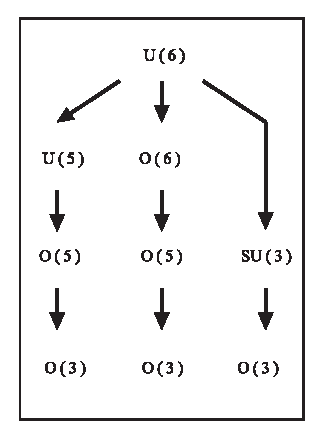
\includegraphics[scale=.65]{figure}
%
% If not, use
%\picplace{5cm}{2cm} % Give the correct figure height and width in cm
%
\caption{If the width of the figure is less than 7.8 cm use the \texttt{sidecapion} command to flush the caption on the left side of the page. If the figure is positioned at the top of the page, align the sidecaption with the top of the figure -- to achieve this you simply need to use the optional argument \texttt{[t]} with the \texttt{sidecaption} command}
\label{fig:1}       % Give a unique label
\end{figure}


\paragraph{Paragraph Heading} %
Instead of simply listing headings of different levels we recommend to let every heading be followed by at least a short passage of text. Furtheron please use the \LaTeX\ automatism for all your cross-references and citations as has already been described in Sect.~\ref{sec:2}.

Please note that the first line of text that follows a heading is not indented, whereas the first lines of all subsequent paragraphs are.

For typesetting numbered lists we recommend to use the \verb|enumerate| environment -- it will automatically render Springer's preferred layout.

\begin{enumerate}
\item{Livelihood and survival mobility are oftentimes coutcomes of uneven socioeconomic development.}
\begin{enumerate}
\item{Livelihood and survival mobility are oftentimes coutcomes of uneven socioeconomic development.}
\item{Livelihood and survival mobility are oftentimes coutcomes of uneven socioeconomic development.}
\end{enumerate}
\item{Livelihood and survival mobility are oftentimes coutcomes of uneven socioeconomic development.}
\end{enumerate}


\subparagraph{Subparagraph Heading} In order to avoid simply listing headings of different levels we recommend to let every heading be followed by at least a short passage of text. Use the \LaTeX\ automatism for all your cross-references and citations as has already been described in Sect.~\ref{sec:2}, see also Fig.~\ref{fig:2}.

Please note that the first line of text that follows a heading is not indented, whereas the first lines of all subsequent paragraphs are.

For unnumbered list we recommend to use the \verb|itemize| environment -- it will automatically render Springer's preferred layout.

\begin{itemize}
\item{Livelihood and survival mobility are oftentimes coutcomes of uneven socioeconomic development, cf. Table~\ref{tab:1}.}
\begin{itemize}
\item{Livelihood and survival mobility are oftentimes coutcomes of uneven socioeconomic development.}
\item{Livelihood and survival mobility are oftentimes coutcomes of uneven socioeconomic development.}
\end{itemize}
\item{Livelihood and survival mobility are oftentimes coutcomes of uneven socioeconomic development.}
\end{itemize}

\begin{figure}[t]
\sidecaption[t]
% Use the relevant command for your figure-insertion program
% to insert the figure file.
% For example, with the option graphics use
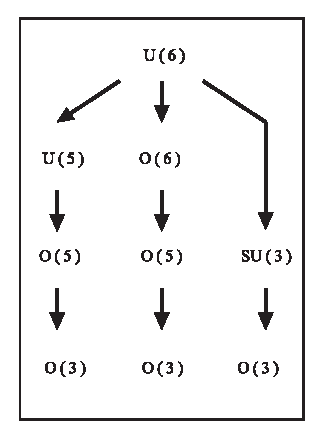
\includegraphics[scale=.65]{figure}
%
% If not, use
%\picplace{5cm}{2cm} % Give the correct figure height and width in cm
%
\caption{Please write your figure caption here}
\label{fig:2}       % Give a unique label
\end{figure}

\runinhead{Run-in Heading Boldface Version} Use the \LaTeX\ automatism for all your cross-references and citations as has already been described in Sect.~\ref{sec:2}.

\subruninhead{Run-in Heading Italic Version} Use the \LaTeX\ automatism for all your cross-refer\-ences and citations as has already been described in Sect.~\ref{sec:2}\index{paragraph}.
% Use the \index{} command to code your index words
%
% For tables use
%
\begin{table}
\caption{Please write your table caption here}
\label{tab:1}       % Give a unique label
%
% For LaTeX tables use
%
\begin{tabular}{p{2cm}p{2.4cm}p{2cm}p{4.9cm}}
\hline\noalign{\smallskip}
Classes & Subclass & Length & Action Mechanism  \\
\noalign{\smallskip}\svhline\noalign{\smallskip}
Translation & mRNA$^a$  & 22 (19--25) & Translation repression, mRNA cleavage\\
Translation & mRNA cleavage & 21 & mRNA cleavage\\
Translation & mRNA  & 21--22 & mRNA cleavage\\
Translation & mRNA  & 24--26 & Histone and DNA Modification\\
\noalign{\smallskip}\hline\noalign{\smallskip}
\end{tabular}
$^a$ Table foot note (with superscript)
\end{table}
%
\section{Section Heading}
\label{sec:3}
% Always give a unique label
% and use \ref{<label>} for cross-references
% and \cite{<label>} for bibliographic references
% use \sectionmark{}
% to alter or adjust the section heading in the running head
Instead of simply listing headings of different levels we recommend to let every heading be followed by at least a short passage of text. Furtheron please use the \LaTeX\ automatism for all your cross-references and citations as has already been described in Sect.~\ref{sec:2}.

Please note that the first line of text that follows a heading is not indented, whereas the first lines of all subsequent paragraphs are.

If you want to list definitions or the like we recommend to use the Springer-enhanced \verb|description| environment -- it will automatically render Springer's preferred layout.

\begin{description}[Type 1]
\item[Type 1]{That addresses central themes pertainng to migration, health, and disease. In Sect.~\ref{sec:1}, Wilson discusses the role of human migration in infectious disease distributions and patterns.}
\item[Type 2]{That addresses central themes pertainng to migration, health, and disease. In Sect.~\ref{subsec:2}, Wilson discusses the role of human migration in infectious disease distributions and patterns.}
\end{description}

\subsection{Subsection Heading} %
In order to avoid simply listing headings of different levels we recommend to let every heading be followed by at least a short passage of text. Use the \LaTeX\ automatism for all your cross-references and citations citations as has already been described in Sect.~\ref{sec:2}.

Please note that the first line of text that follows a heading is not indented, whereas the first lines of all subsequent paragraphs are.

\begin{svgraybox}
If you want to emphasize complete paragraphs of texts we recommend to use the newly defined Springer class option \verb|graybox| and the newly defined environment \verb|svgraybox|. This will produce a 15 percent screened box 'behind' your text.

If you want to emphasize complete paragraphs of texts we recommend to use the newly defined Springer class option and environment \verb|svgraybox|. This will produce a 15 percent screened box 'behind' your text.
\end{svgraybox}


\subsubsection{Subsubsection Heading}
Instead of simply listing headings of different levels we recommend to let every heading be followed by at least a short passage of text. Furtheron please use the \LaTeX\ automatism for all your cross-references and citations as has already been described in Sect.~\ref{sec:2}.

Please note that the first line of text that follows a heading is not indented, whereas the first lines of all subsequent paragraphs are.

\begin{theorem}
Theorem text goes here.
\end{theorem}
%
% or
%
\begin{definition}
Definition text goes here.
\end{definition}

\begin{proof}
%\smartqed
Proof text goes here.
\qed
\end{proof}

\paragraph{Paragraph Heading} %
Instead of simply listing headings of different levels we recommend to let every heading be followed by at least a short passage of text. Furtheron please use the \LaTeX\ automatism for all your cross-references and citations as has already been described in Sect.~\ref{sec:2}.

Note that the first line of text that follows a heading is not indented, whereas the first lines of all subsequent paragraphs are.
%
% For built-in environments use
%
\begin{theorem}
Theorem text goes here.
\end{theorem}
%
\begin{definition}
Definition text goes here.
\end{definition}
%
\begin{proof}
\smartqed
Proof text goes here.
\qed
\end{proof}
%
\begin{acknowledgement}
If you want to include acknowledgments of assistance and the like at the end of an individual chapter please use the \verb|acknowledgement| environment -- it will automatically render Springer's preferred layout.
\end{acknowledgement}
%
\section*{Appendix}
\addcontentsline{toc}{section}{Appendix}
%
When placed at the end of a chapter or contribution (as opposed to at the end of the book), the numbering of tables, figures, and equations in the appendix section continues on from that in the main text. Hence please \textit{do not} use the \verb|appendix| command when writing an appendix at the end of your chapter or contribution. If there is only one the appendix is designated ``Appendix'', or ``Appendix 1'', or ``Appendix 2'', etc. if there is more than one.

\begin{equation}
a \times b = c
\end{equation}
% Problems or Exercises should be sorted chapterwise
\section*{Problems}
\addcontentsline{toc}{section}{Problems}
%
% Use the following environment.
% Don't forget to label each problem;
% the label is needed for the solutions' environment
\begin{prob}
\label{prob1}
A given problem or Excercise is described here. The
problem is described here. The problem is described here.
\end{prob}

\begin{prob}
\label{prob2}
\textbf{Problem Heading}\\
(a) The first part of the problem is described here.\\
(b) The second part of the problem is described here.
\end{prob}

%%%%%%%%%%%%%%%%%%%%%%%% referenc.tex %%%%%%%%%%%%%%%%%%%%%%%%%%%%%%
% sample references
% %
% Use this file as a template for your own input.
%
%%%%%%%%%%%%%%%%%%%%%%%% Springer-Verlag %%%%%%%%%%%%%%%%%%%%%%%%%%
%
% BibTeX users please use
% \bibliographystyle{}
% \bibliography{}
%
\biblstarthook{In view of the parallel print and (chapter-wise) online publication of your book at \url{www.springerlink.com} it has been decided that -- as a genreral rule --  references should be sorted chapter-wise and placed at the end of the individual chapters. However, upon agreement with your contact at Springer you may list your references in a single seperate chapter at the end of your book. Deactivate the class option \texttt{sectrefs} and the \texttt{thebibliography} environment will be put out as a chapter of its own.\\\indent
References may be \textit{cited} in the text either by number (preferred) or by author/year.\footnote{Make sure that all references from the list are cited in the text. Those not cited should be moved to a separate \textit{Further Reading} section or chapter.} The reference list should ideally be \textit{sorted} in alphabetical order -- even if reference numbers are used for the their citation in the text. If there are several works by the same author, the following order should be used: 
\begin{enumerate}
\item all works by the author alone, ordered chronologically by year of publication
\item all works by the author with a coauthor, ordered alphabetically by coauthor
\item all works by the author with several coauthors, ordered chronologically by year of publication.
\end{enumerate}
The \textit{styling} of references\footnote{Always use the standard abbreviation of a journal's name according to the ISSN \textit{List of Title Word Abbreviations}, see \url{http://www.issn.org/2-22661-LTWA-online.php}} depends on the subject of your book:
\begin{itemize}
\item The \textit{two} recommended styles for references in books on \textit{mathematical, physical, statistical and computer sciences} are depicted in ~\cite{science-contrib, science-online, science-mono, science-journal, science-DOI} and ~\cite{phys-online, phys-mono, phys-journal, phys-DOI, phys-contrib}.
\item Examples of the most commonly used reference style in books on \textit{Psychology, Social Sciences} are~\cite{psysoc-mono, psysoc-online,psysoc-journal, psysoc-contrib, psysoc-DOI}.
\item Examples for references in books on \textit{Humanities, Linguistics, Philosophy} are~\cite{humlinphil-journal, humlinphil-contrib, humlinphil-mono, humlinphil-online, humlinphil-DOI}.
\item Examples of the basic Springer style used in publications on a wide range of subjects such as \textit{Computer Science, Economics, Engineering, Geosciences, Life Sciences, Medicine, Biomedicine} are ~\cite{basic-contrib, basic-online, basic-journal, basic-DOI, basic-mono}. 
\end{itemize}
}

\begin{thebibliography}{99.}%
% and use \bibitem to create references.
%
% Use the following syntax and markup for your references if 
% the subject of your book is from the field 
% "Mathematics, Physics, Statistics, Computer Science"
%
% Contribution 
\bibitem{science-contrib} Broy, M.: Software engineering --- from auxiliary to key technologies. In: Broy, M., Dener, E. (eds.) Software Pioneers, pp. 10-13. Springer, Heidelberg (2002)
%
% Online Document
\bibitem{science-online} Dod, J.: Effective substances. In: The Dictionary of Substances and Their Effects. Royal Society of Chemistry (1999) Available via DIALOG. \\
\url{http://www.rsc.org/dose/title of subordinate document. Cited 15 Jan 1999}
%
% Monograph
\bibitem{science-mono} Geddes, K.O., Czapor, S.R., Labahn, G.: Algorithms for Computer Algebra. Kluwer, Boston (1992) 
%
% Journal article
\bibitem{science-journal} Hamburger, C.: Quasimonotonicity, regularity and duality for nonlinear systems of partial differential equations. Ann. Mat. Pura. Appl. \textbf{169}, 321--354 (1995)
%
% Journal article by DOI
\bibitem{science-DOI} Slifka, M.K., Whitton, J.L.: Clinical implications of dysregulated cytokine production. J. Mol. Med. (2000) doi: 10.1007/s001090000086 
%
\bigskip

% Use the following (APS) syntax and markup for your references if 
% the subject of your book is from the field 
% "Mathematics, Physics, Statistics, Computer Science"
%
% Online Document
\bibitem{phys-online} J. Dod, in \textit{The Dictionary of Substances and Their Effects}, Royal Society of Chemistry. (Available via DIALOG, 1999), 
\url{http://www.rsc.org/dose/title of subordinate document. Cited 15 Jan 1999}
%
% Monograph
\bibitem{phys-mono} H. Ibach, H. L\"uth, \textit{Solid-State Physics}, 2nd edn. (Springer, New York, 1996), pp. 45-56 
%
% Journal article
\bibitem{phys-journal} S. Preuss, A. Demchuk Jr., M. Stuke, Appl. Phys. A \textbf{61}
%
% Journal article by DOI
\bibitem{phys-DOI} M.K. Slifka, J.L. Whitton, J. Mol. Med., doi: 10.1007/s001090000086
%
% Contribution 
\bibitem{phys-contrib} S.E. Smith, in \textit{Neuromuscular Junction}, ed. by E. Zaimis. Handbook of Experimental Pharmacology, vol 42 (Springer, Heidelberg, 1976), p. 593
%
\bigskip
%
% Use the following syntax and markup for your references if 
% the subject of your book is from the field 
% "Psychology, Social Sciences"
%
%
% Monograph
\bibitem{psysoc-mono} Calfee, R.~C., \& Valencia, R.~R. (1991). \textit{APA guide to preparing manuscripts for journal publication.} Washington, DC: American Psychological Association.
%
% Online Document
\bibitem{psysoc-online} Dod, J. (1999). Effective substances. In: The dictionary of substances and their effects. Royal Society of Chemistry. Available via DIALOG. \\
\url{http://www.rsc.org/dose/Effective substances.} Cited 15 Jan 1999.
%
% Journal article
\bibitem{psysoc-journal} Harris, M., Karper, E., Stacks, G., Hoffman, D., DeNiro, R., Cruz, P., et al. (2001). Writing labs and the Hollywood connection. \textit{J Film} Writing, 44(3), 213--245.
%
% Contribution 
\bibitem{psysoc-contrib} O'Neil, J.~M., \& Egan, J. (1992). Men's and women's gender role journeys: Metaphor for healing, transition, and transformation. In B.~R. Wainrig (Ed.), \textit{Gender issues across the life cycle} (pp. 107--123). New York: Springer.
%
% Journal article by DOI
\bibitem{psysoc-DOI}Kreger, M., Brindis, C.D., Manuel, D.M., Sassoubre, L. (2007). Lessons learned in systems change initiatives: benchmarks and indicators. \textit{American Journal of Community Psychology}, doi: 10.1007/s10464-007-9108-14.
%
%
% Use the following syntax and markup for your references if 
% the subject of your book is from the field 
% "Humanities, Linguistics, Philosophy"
%
\bigskip
%
% Journal article
\bibitem{humlinphil-journal} Alber John, Daniel C. O'Connell, and Sabine Kowal. 2002. Personal perspective in TV interviews. \textit{Pragmatics} 12:257--271
%
% Contribution 
\bibitem{humlinphil-contrib} Cameron, Deborah. 1997. Theoretical debates in feminist linguistics: Questions of sex and gender. In \textit{Gender and discourse}, ed. Ruth Wodak, 99--119. London: Sage Publications.
%
% Monograph
\bibitem{humlinphil-mono} Cameron, Deborah. 1985. \textit{Feminism and linguistic theory.} New York: St. Martin's Press.
%
% Online Document
\bibitem{humlinphil-online} Dod, Jake. 1999. Effective substances. In: The dictionary of substances and their effects. Royal Society of Chemistry. Available via DIALOG. \\
http://www.rsc.org/dose/title of subordinate document. Cited 15 Jan 1999
%
% Journal article by DOI
\bibitem{humlinphil-DOI} Suleiman, Camelia, Daniel C. O�Connell, and Sabine Kowal. 2002. `If you and I, if we, in this later day, lose that sacred fire...�': Perspective in political interviews. \textit{Journal of Psycholinguistic Research}. doi: 10.1023/A:1015592129296.
%
%
%
\bigskip
%
%
% Use the following syntax and markup for your references if 
% the subject of your book is from the field 
% "Computer Science, Economics, Engineering, Geosciences, Life Sciences"
%
%
% Contribution 
\bibitem{basic-contrib} Brown B, Aaron M (2001) The politics of nature. In: Smith J (ed) The rise of modern genomics, 3rd edn. Wiley, New York 
%
% Online Document
\bibitem{basic-online} Dod J (1999) Effective Substances. In: The dictionary of substances and their effects. Royal Society of Chemistry. Available via DIALOG. \\
\url{http://www.rsc.org/dose/title of subordinate document. Cited 15 Jan 1999}
%
% Journal article by DOI
\bibitem{basic-DOI} Slifka MK, Whitton JL (2000) Clinical implications of dysregulated cytokine production. J Mol Med, doi: 10.1007/s001090000086
%
% Journal article
\bibitem{basic-journal} Smith J, Jones M Jr, Houghton L et al (1999) Future of health insurance. N Engl J Med 965:325--329
%
% Monograph
\bibitem{basic-mono} South J, Blass B (2001) The future of modern genomics. Blackwell, London 
%
\end{thebibliography}


%%%%%%%%%%%%%%%%%%%%% appendix.tex %%%%%%%%%%%%%%%%%%%%%%%%%%%%%%%%%
%
% sample appendix
%
% Use this file as a template for your own input.
%
%%%%%%%%%%%%%%%%%%%%%%%% Springer-Verlag %%%%%%%%%%%%%%%%%%%%%%%%%%

\appendix
\motto{All's well that ends well}
\chapter{Chapter Heading}
\label{introA} % Always give a unique label
% use \chaptermark{}
% to alter or adjust the chapter heading in the running head

Use the template \emph{appendix.tex} together with the Springer document class SVMono (monograph-type books) or SVMult (edited books) to style appendix of your book in the Springer layout.


\section{Section Heading}
\label{sec:A1}
% Always give a unique label
% and use \ref{<label>} for cross-references
% and \cite{<label>} for bibliographic references
% use \sectionmark{}
% to alter or adjust the section heading in the running head
Instead of simply listing headings of different levels we recommend to let every heading be followed by at least a short passage of text. Furtheron please use the \LaTeX\ automatism for all your cross-references and citations.


\subsection{Subsection Heading}
\label{sec:A2}
Instead of simply listing headings of different levels we recommend to let every heading be followed by at least a short passage of text. Furtheron please use the \LaTeX\ automatism for all your cross-references and citations as has already been described in Sect.~\ref{sec:A1}.

For multiline equations we recommend to use the \verb|eqnarray| environment.
\begin{eqnarray}
\vec{a}\times\vec{b}=\vec{c} \nonumber\\
\vec{a}\times\vec{b}=\vec{c}
\label{eq:A01}
\end{eqnarray}

\subsubsection{Subsubsection Heading}
Instead of simply listing headings of different levels we recommend to let every heading be followed by at least a short passage of text. Furtheron please use the \LaTeX\ automatism for all your cross-references and citations as has already been described in Sect.~\ref{sec:A2}.

Please note that the first line of text that follows a heading is not indented, whereas the first lines of all subsequent paragraphs are.

% For figures use
%
\begin{figure}[t]
\sidecaption[t]
%\centering
% Use the relevant command for your figure-insertion program
% to insert the figure file.
% For example, with the option graphics use
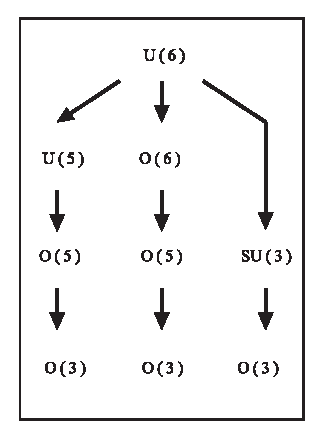
\includegraphics[scale=.65]{figure}
%
% If not, use
%\picplace{5cm}{2cm} % Give the correct figure height and width in cm
%
\caption{Please write your figure caption here}
\label{fig:A1}       % Give a unique label
\end{figure}

% For tables use
%
\begin{table}
\caption{Please write your table caption here}
\label{tab:A1}       % Give a unique label
%
% For LaTeX tables use
%
\begin{tabular}{p{2cm}p{2.4cm}p{2cm}p{4.9cm}}
\hline\noalign{\smallskip}
Classes & Subclass & Length & Action Mechanism  \\
\noalign{\smallskip}\hline\noalign{\smallskip}
Translation & mRNA$^a$  & 22 (19--25) & Translation repression, mRNA cleavage\\
Translation & mRNA cleavage & 21 & mRNA cleavage\\
Translation & mRNA  & 21--22 & mRNA cleavage\\
Translation & mRNA  & 24--26 & Histone and DNA Modification\\
\noalign{\smallskip}\hline\noalign{\smallskip}
\end{tabular}
$^a$ Table foot note (with superscript)
\end{table}
%


\backmatter%%%%%%%%%%%%%%%%%%%%%%%%%%%%%%%%%%%%%%%%%%%%%%%%%%%%%%%
%%
%% This is file `glossary.sty',
%% generated with the docstrip utility.
%%
%% The original source files were:
%%
%% glossary.dtx  (with options: `glossary.sty,package')
%% Copyright (C) 2006 Nicola Talbot, all rights reserved.
%% If you modify this file, you must change its name first.
%% You are NOT ALLOWED to distribute this file alone. You are NOT
%% ALLOWED to take money for the distribution or use of either this
%% file or a changed version, except for a nominal charge for copying
%% etc.
%% \CharacterTable
%%  {Upper-case    \A\B\C\D\E\F\G\H\I\J\K\L\M\N\O\P\Q\R\S\T\U\V\W\X\Y\Z
%%   Lower-case    \a\b\c\d\e\f\g\h\i\j\k\l\m\n\o\p\q\r\s\t\u\v\w\x\y\z
%%   Digits        \0\1\2\3\4\5\6\7\8\9
%%   Exclamation   \!     Double quote  \"     Hash (number) \#
%%   Dollar        \$     Percent       \%     Ampersand     \&
%%   Acute accent  \'     Left paren    \(     Right paren   \)
%%   Asterisk      \*     Plus          \+     Comma         \,
%%   Minus         \-     Point         \.     Solidus       \/
%%   Colon         \:     Semicolon     \;     Less than     \<
%%   Equals        \=     Greater than  \>     Question mark \?
%%   Commercial at \@     Left bracket  \[     Backslash     \\
%%   Right bracket \]     Circumflex    \^     Underscore    \_
%%   Grave accent  \`     Left brace    \{     Vertical bar  \|
%%   Right brace   \}     Tilde         \~}
\NeedsTeXFormat{LaTeX2e}
\ProvidesPackage{glossary}[2006/07/20 2.4 (NLCT)]
\RequirePackage{ifthen}
\RequirePackage{keyval}
\define@key{gloss}
{style}
{\ifthenelse{\equal{#1}{list} \or \equal{#1}{altlist}
\or \equal{#1}{super} \or \equal{#1}{long}}
{\def\gls@style{#1}}
{\PackageError{glossary}
{Unknown glossary style '#1'}
{Available styles are: list, altlist, super and long}}}
\define@key{gloss}
{header}[plain]{\ifthenelse{\equal{#1}{none} \or \equal{#1}{plain}}
{\def\gls@header{#1}}
{\PackageError{glossary}
{Unknown glossary style '#1'}
{Available styles are: none and plain}}}
\define@key{gloss}
{border}[plain]{\ifthenelse{\equal{#1}{none} \or \equal{#1}{plain}}
{\def\gls@border{#1}}
{\PackageError{glossary}
{Unknown glossary border '#1'}
{Available styles are: none and plain}}}
\newcount\gls@cols
\define@key{gloss}{cols}{\gls@cols=#1\relax
\ifthenelse{\gls@cols<2 \or \gls@cols>3}
{\PackageError{glossary}
{invalid number of columns}
{The cols option can only be 2 or 3}}
{}}
\define@key{gloss}
{number}
{\ifthenelse{\equal{#1}{none}}
{\def\gls@glossary@number{#1}}
{\@ifundefined{c@#1}{
\PackageError{glossary}
{Unknown glossary number style '#1'}
{You may either specify "none" or the name of a counter,
e.g. "section"}\def\gls@glossary@number{page}}{\def\gls@glossary@number{#1}}}}
\newif\ifgls@toc
\define@key{gloss}{toc}[true]{\ifthenelse{\equal{#1}{true}
\or \equal{#1}{false}}
{\csname gls@toc#1\endcsname}
{\PackageError{glossary}{Glossary option 'toc' is boolean}
{The value of 'toc' can only be set to 'true' or 'false'}}}
\newif\ifgls@hypertoc
\define@key{gloss}{hypertoc}[true]{%
\ifthenelse{\equal{#1}{true} \or \equal{#1}{false}}
{\csname gls@hypertoc#1\endcsname}
{\PackageError{glossary}{Glossary option 'hypertoc' is boolean}
{The value of 'hypertoc' can only be set to 'true' or 'false'}}}
\newif\ifgls@section
\define@key{gloss}{section}[true]{%
\ifthenelse{\equal{#1}{true} \or \equal{#1}{false}}
{\csname gls@section#1\endcsname}
{\PackageError{glossary}{Glossary option 'section' is boolean}
{The value of 'section' can only be set to 'true' or 'false'}}}
\gls@sectionfalse
\newif\ifglshyper
\newif\ifglshyperacronym
\define@key{gloss}{hyper}[true]{%
\ifthenelse{\equal{#1}{true} \or \equal{#1}{false}}
{\csname glshyper#1\endcsname\glshyperacronymtrue}
{\PackageError{glossary}{Glossary option 'hyper' is boolean}
{The value of 'hyper' can only be set to 'true' or 'false'}}}
\define@key{gloss}{hyperacronym}[true]{%
\ifthenelse{\equal{#1}{true} \or \equal{#1}{false}}
{\csname glshyperacronym#1\endcsname}
{\PackageError{glossary}{Glossary option 'hyperacronym' is boolean}
{The value of 'hyperacronym' can only be set to 'true' or 'false'}}}
\newif\ifglsacronym
\define@key{gloss}{acronym}[true]{%
\ifthenelse{\equal{#1}{true} \or \equal{#1}{false}}
{\setboolean{glsacronym}{#1}}{%
\PackageError{glossary}{Glossary option 'acronym' is boolean}{The
value of 'acronym' can only be set to 'true' or 'false'}}}
\newif\ifglsglobal
\define@key{gloss}{global}[true]{\ifthenelse{\equal{#1}{true}\or
\equal{#1}{false}}{\setboolean{glsglobal}{#1}}{%
\PackageError{glossary}{Glossary option 'global' is boolean}{The
value of 'global' can only be set to 'true' or 'false'}}}
\def\gls@style{long}
\def\gls@header{none}
\def\gls@border{none}
\def\gls@glossary@number{page}
\gls@cols=2\relax
\gls@tocfalse
\@ifundefined{hyperpage}{\glshyperfalse\glshyperacronymfalse}{%
\glshypertrue\glshyperacronymtrue}
\@ifundefined{hypertarget}{
\newcommand{\glosslabel}[2]{#2}%
\newcommand{\glossref}[2]{#2}%
}{%
\newcommand{\glosslabel}[2]{\hypertarget{#1}{#2}}%
\newcommand{\glossref}[2]{\hyperlink{#1}{#2}}
}
\@ifundefined{xspace}{%
\let\glsxspace\relax}{%
\let\glsxspace\xspace}
\let\glossaryalignment\relax
\newcommand{\glossarypackageoptions}[1]{\setkeys{gloss}{#1}}
\InputIfFileExists{glossary.cfg}{%
\typeout{Glossary configuration file loaded}}{%
\typeout{No configuration file glossary.cfg found}}
\renewcommand{\glossarypackageoptions}[1]{%
\PackageError{glossary}{Command \string\glossarypackageoptions
^^Jcan only be used in configuration file}{}}
\DeclareOption*{\edef\@pkg@ptions{\noexpand
\setkeys{gloss}{\CurrentOption}}
\ifthenelse{\equal{\CurrentOption}{}}{}{\@pkg@ptions}}
\ProcessOptions
\ifthenelse{\(\equal{\gls@style}{list} \or
\equal{\gls@style}{altlist}\) \and
\(\not\equal{\gls@header}{none} \or \not\equal{\gls@border}{none}
\or \gls@cols=3\)}
{\PackageError{glossary}{You can't have option 'style=list' or
'style=altlist' in combination with any of the other style
options}{The 'list' and 'altlist' options don't have a header,
border or number of columns option.}}
{}
\ifthenelse{\boolean{gls@hypertoc} \and \boolean{gls@toc}}{%
\PackageWarning{glossary}{Can't have both 'toc' and
'hypertoc', ignoring 'toc' option}
\ifgls@hypertoc\gls@tocfalse\fi}{}
\define@key{wrgloss}{name}{%
\def\@glo@n@me{#1}%
\@onelevel@sanitize\@glo@n@me%
\global\let\@glo@n@me\@glo@n@me}
\define@key{wrgloss}{description}{%
\def\@descr{#1}%
\@onelevel@sanitize\@descr}
\define@key{wrgloss}{sort}{%
\def\@s@rt{#1}%
\@onelevel@sanitize\@s@rt
\global\let\@s@rt\@s@rt}
\define@key{wrgloss}{format}{\def\@f@rm@t{#1}}
\define@key{wrgloss}{number}{\def\@glo@num{#1}}
\newcommand{\@@wrglossary}{}
\newcommand{\@glo@l@bel}{}
\newcommand{\@gls@glossary@type}{glo}
\renewcommand{\@wrglossary}[2][glossary]{\relax
\gdef\@glo@n@me{}\def\@descr{}\def\@s@rt{}\def\@f@rm@t{}%
\edef\@glo@num{\csname gls@#1@number\endcsname}\relax
\xdef\@pr@fix{\csname @gls@#1@type\endcsname}%
 \setkeys{wrgloss}{#2}\relax
\ifthenelse{\equal{\@glo@num}{none}}{\def\@@glo@num{\thepage}}{%
\@ifundefined{c@\@glo@num}{\PackageError{glossary}{%
Not such counter '\@glo@num'}{The value of the 'number' key
must be the name of a counter or the word "none"}%
\def\@@glo@num{\thepage}}{%
\edef\@@glo@num{\csname the\@glo@num\endcsname}}}%
\ifthenelse{\equal{\@s@rt}{}}{\gdef\@s@rt{\@glo@n@me}}{}%
\ifthenelse{\equal{\@glo@l@bel}{}}{%
\gdef\@glo@l@bel{\@pr@fix:\@s@rt}}{}%
\ifthenelse{\equal{\@f@rm@t}{}}
{\expandafter\protected@write\csname @#1file\endcsname{}%
{\string\glossaryentry{\@s@rt @{%
\string\glosslabel{\@glo@l@bel}{\@glo@n@me}}\@descr
\string\relax|glsnumformat}{\@@glo@num}}}
{\ifthenelse{\equal{\@f@rm@t}{hyperrm} \or
\equal{\@f@rm@t}{hypersf} \or \equal{\@f@rm@t}{hypertt}
\or \equal{\@f@rm@t}{hypermd} \or \equal{\@f@rm@t}{hyperbf}
\or \equal{\@f@rm@t}{hyperit} \or \equal{\@f@rm@t}{hyperem}
\or \equal{\@f@rm@t}{hypersl} \or \equal{\@f@rm@t}{hyperup}
\or \equal{\@f@rm@t}{hypersc}}
{\expandafter\protected@write\csname @#1file\endcsname{}%
    {\string\glossaryentry{\@s@rt @{%
     \string\glosslabel{\@glo@l@bel}{\@glo@n@me}}\@descr
     \string\relax|\@f@rm@t[\@glo@num]}{\@@glo@num}}}
{\expandafter\protected@write\csname @#1file\endcsname{}%
    {\string\glossaryentry{\@s@rt @{%
     \string\glosslabel{\@glo@l@bel}{\@glo@n@me}}\@descr
     \string\relax|\@f@rm@t}{\@@glo@num}}}}\relax
 \endgroup\@esphack
\@@wrglossary
}
\define@key{wrnsgloss}{name}{\def\@glo@n@me{#1}}
\define@key{wrnsgloss}{description}{\def\@descr{#1}}
\define@key{wrnsgloss}{sort}{\def\@s@rt{#1}}
\define@key{wrnsgloss}{format}{\def\@f@rm@t{#1}}
\define@key{wrnsgloss}{number}{\def\@glo@num{#1}}
\newcommand{\@gls@getn@me}[1]{%
\def\@glo@n@me{}\setkeys{wrnsgloss}{#1}%
}
\newcommand{\@gls@getdescr}[1]{%
\@bsphack\begingroup
\def\@descr{}%
\setkeys{wrgloss}{#1}%
\global\let\@glo@desc\@descr
\endgroup\@esphack
}
\newcommand{\xglossary}{\renewcommand{\@@wrglossary}[1]{%
\glossref{\@glo@l@bel}{##1}\renewcommand{\@@wrglossary}{}}%
\glossary}
\newcommand*{\@glo@label@list}{}
\toksdef\gls@ta=0 \toksdef\gls@tb=2
\newcommand{\@glo@label@addtolist}[1]{%
\gls@ta={{#1}}\gls@tb=\expandafter{\@glo@label@list}%
\xdef\@glo@label@list{\the\gls@ta,\the\gls@tb}}
\newcommand*{\storeglosentry}[3][glossary]{%
\ifthenelse{\equal{#2}{*}}{%
\PackageError{glossary}{Glossary label '*' invalid}{You can't have
a glossary entry with a * as the label}}{%
\@ifundefined{glo@#2@entry}{%
\@glo@label@addtolist{#2}%
\expandafter\def\csname glo@#2@type\endcsname{#1}%
\expandafter\def\csname glo@#2@entry\endcsname{#3}%
\@gls@getn@me{#3}%
\expandafter\protected@edef\csname glo@#2@name\endcsname{\@glo@n@me}%
}{%
\PackageError{glossary}{Glossary entry '#2' already
defined}{There already exists a glossary entry with the label '#2'}}}%
}
\providecommand{\useglosentry}[2][\relax]{%
\ifthenelse{\equal{#2}{*}}{\@for\@glolab:=\@glo@label@list\do{%
\ifthenelse{\equal{\@glolab}{}}{}{\useglosentry[#1]{\@glolab}}}}{%
\@ifundefined{glo@#2@type}{%
\PackageError{glossary}{Glossary entry '#2' undefined}{You need
to define the entry using \string\storeglosentry\space before
using it.}}{{%
\edef\@glostype{\csname glo@#2@type\endcsname}%
\@glo@tb=\expandafter\expandafter\expandafter
{\csname glo@#2@entry\endcsname}%
\ifx#1\relax
\edef\@glo@cmd{\expandafter\noexpand
\csname\@glostype\endcsname{\the\@glo@tb}}%
\else
\edef\@glo@cmd{\expandafter\noexpand
\csname\@glostype\endcsname{\the\@glo@tb,#1}}%
\fi
\@glo@cmd
}}}}
\providecommand{\useGlosentry}[3][\relax]{%
\@ifundefined{glo@#2@type}{%
\PackageError{glossary}{Glossary entry '#2' undefined}{You need
to define the entry using \string\storeglosentry\space before
using it.}}{{%
\edef\@glostype{x\csname glo@#2@type\endcsname}%
\@glo@tb=\expandafter\expandafter\expandafter
{\csname glo@#2@entry\endcsname}%
\ifx#1\relax
\edef\@glo@cmd{\expandafter\noexpand
\csname\@glostype\endcsname{\the\@glo@tb}}%
\else
\edef\@glo@cmd{\expandafter\noexpand
\csname\@glostype\endcsname{\the\@glo@tb,#1}}%
\fi
\@glo@cmd{#3}%
}}}
\newcommand{\gls}[2][\relax]{%
\useGlosentry[#1]{#2}{%
\csname glo@#2@name\endcsname}}
\providecommand{\saveglosentry}[3][glossary]{%
\PackageWarning{glossary}{\string\saveglosentry\space is obsolete,
please use \string\storeglosentry\space instead}%
\expandafter\def\csname glo@#2@type\endcsname{#1}%
\expandafter\def\csname glo@#2@entry\endcsname{%
name={#2},description={#3}}}
\newcommand*{\@gls@setnumbering}[2][glossary]{%
\ifthenelse{\equal{#2}{none}}{%
\def\pagecompositor{-}
\expandafter\def\csname @#1@delimN\endcsname{}
\expandafter\def\csname @#1@delimR\endcsname{}
\expandafter\def\csname glsX#1Xnumformat\endcsname##1{}}{%
\ifthenelse{\equal{#2}{page}}{%
\def\pagecompositor{-}}{%
\def\pagecompositor{.}}
\expandafter\def\csname @#1@delimN\endcsname{, }
\expandafter\def\csname @#1@delimR\endcsname{--}
\ifglshyper
\expandafter\def\csname glsX#1Xnumformat\endcsname##1{%
\hyperrm[#2]{##1}}%
\else
\expandafter\def\csname glsX#1Xnumformat\endcsname##1{##1}\fi
}
}
\@gls@setnumbering{\gls@glossary@number}
\newcommand{\glsnumformat}[1]{%
\@ifundefined{\@glostype}{\def\@glostype{glossary}}{}%
\@ifundefined{glsX\@glostype Xnumformat}{%
\PackageError{glossary}{Glossary type '\@glostype' undefined}{}}{%
\csname glsX\@glostype Xnumformat\endcsname{#1}}}
\def\@glostype{glossary}
\newcommand{\delimN}{\csname @\@glostype @delimN\endcsname}
\newcommand{\delimR}{\csname @\@glostype @delimR\endcsname}
\newcommand{\gloitem}{\csname @\@glostype @gloitem\endcsname}
\newcommand{\gloskip}{\csname @\@glostype @gloskip\endcsname}
\newcommand{\delimT}{\glsafternum
\csname @\@glostype @delimT\endcsname}
\newcommand{\glodelim}{\csname @\@glostype @glodelim\endcsname
\glsbeforenum}
\newcommand{\glogroupSymbols}{}
\newcommand{\glogroupNumbers}{}
\newcommand{\glogroupA}{}
\newcommand{\glogroupB}{}
\newcommand{\glogroupC}{}
\newcommand{\glogroupD}{}
\newcommand{\glogroupE}{}
\newcommand{\glogroupF}{}
\newcommand{\glogroupG}{}
\newcommand{\glogroupH}{}
\newcommand{\glogroupI}{}
\newcommand{\glogroupJ}{}
\newcommand{\glogroupK}{}
\newcommand{\glogroupL}{}
\newcommand{\glogroupM}{}
\newcommand{\glogroupN}{}
\newcommand{\glogroupO}{}
\newcommand{\glogroupP}{}
\newcommand{\glogroupQ}{}
\newcommand{\glogroupR}{}
\newcommand{\glogroupS}{}
\newcommand{\glogroupT}{}
\newcommand{\glogroupU}{}
\newcommand{\glogroupV}{}
\newcommand{\glogroupW}{}
\newcommand{\glogroupX}{}
\newcommand{\glogroupY}{}
\newcommand{\glogroupZ}{}
\define@key{glossnum}{glsnumformat}{\def\@glsnumformat{#1}}
\define@key{glossnum}{type}{\def\@glsnumtype{#1}}
\define@key{glossnum}{delimN}{\def\@delimN{#1}}
\define@key{glossnum}{delimR}{\def\@delimR{#1}}
\define@key{glossnum}{delimT}{\def\@delimT{#1}}
\define@key{glossnum}{gloskip}{\def\@gloskip{#1}}
\define@key{glossnum}{glodelim}{\def\@glodelim{#1}}
\providecommand{\ignore}[1]{}
\newcommand{\setglossary}[1]{%
\def\@glsnumformat{}%
\def\@glsnumtype{glossary}%
\def\@delimN{@dontchange@}%
\def\@delimR{@dontchange@}%
\def\@delimT{@dontchange@}%
\def\@gloskip{@dontchange@}%
\def\@glodelim{@dontchange@}%
\setkeys{glossnum}{#1}\relax
\@ifundefined{print\@glsnumtype}{%
\PackageError{glossary}{Invalid glossary type '\@glsnumtype'}{%
Glossary type '\@glsnumtype' has not been defined}
}{%
\ifthenelse{\equal{\@glsnumformat}{}}{}{%
\expandafter\xdef\csname glsX\@glsnumtype Xnumformat\endcsname{%
\noexpand\csname\@glsnumformat\noexpand\endcsname}%
\ifthenelse{\equal{\@glsnumformat}{ignore}}{%
\expandafter\xdef\csname @\@glsnumtype @delimN\endcsname{}%
\expandafter\xdef\csname @\@glsnumtype @delimR\endcsname{}%
}{}%
}%
\ifthenelse{\equal{\@delimN}{@dontchange@}}{}{%
\expandafter\xdef\csname @\@glsnumtype @delimN\endcsname{%
\@delimN}}%
\ifthenelse{\equal{\@delimR}{@dontchange@}}{}{%
\expandafter\xdef\csname @\@glsnumtype @delimR\endcsname{%
\@delimR}}%
\ifthenelse{\equal{\@delimT}{@dontchange@}}{}{%
\expandafter\xdef\csname @\@glsnumtype @delimT\endcsname{%
\@delimT}}%
\ifthenelse{\equal{\@gloskip}{@dontchange@}}{}{%
\expandafter\xdef\csname @\@glsnumtype @gloskip\endcsname{%
\@gloskip}}%
\ifthenelse{\equal{\@glodelim}{@dontchange@}}{}{%
\expandafter\xdef\csname @\@glsnumtype @glodelim\endcsname{%
\@glodelim}%
}%
}}
\newcommand{\@gls@glossary@inext}{gls}
\newcommand\printglossary[1][glossary]{%
\def\@glostype{#1}%
\@ifundefined{#1name}{%
\renewcommand{\@glossaryname}{\glossaryname}}{%
\renewcommand{\@glossaryname}{\csname #1name\endcsname}}%
\@ifundefined{short#1name}{%
\renewcommand{\@shortglossaryname}{\@glossaryname}}{%
\renewcommand{\@shortglossaryname}{\csname short#1name\endcsname}}%
\expandafter\let\expandafter\gls@number\csname gls@#1@number\endcsname
\@input@{\jobname.\csname @gls@#1@inext\endcsname}}
\providecommand{\glossaryname}{Glossary}
\newcommand{\shortglossaryname}{\glossaryname}
\newcommand{\entryname}{Notation}
\newcommand{\descriptionname}{Description}
\newcommand{\istfilename}{\jobname.ist}
\def\@glossaryname{\glossaryname}
\def\@shortglossaryname{\shortglossaryname}
\newcommand{\@istfilename}[1]{}
\providecommand{\glossarytitle}{%
\@ifundefined{chapter}%
{%
\ifgls@hypertoc
\phantomsection
\@glosaddtoc{section}%
\section*{\@glossaryname}\relax
\else
\section*{\@glossaryname}\relax
\ifgls@toc\@glosaddtoc{section}\fi
\fi}%
{%
\ifthenelse{\boolean{gls@section}}%
{%
\ifgls@hypertoc
\phantomsection
\@glosaddtoc{section}%
\section*{\@glossaryname}\relax
\else
\section*{\@glossaryname}\relax
\ifgls@toc\@glosaddtoc{section}\fi
\fi}%
{%
\ifgls@hypertoc
\@ifundefined{if@twoside}{%
\clearpage}{%
\if@twoside
\@ifundefined{cleardoublepage}{\clearpage}{\cleardoublepage}%
\else
\clearpage
\fi}%
\phantomsection
\@glosaddtoc{chapter}%
\fi
\chapter*{\@glossaryname}\relax
\ifgls@toc\@glosaddtoc{chapter}\fi}}
\markboth{\@shortglossaryname}{\@shortglossaryname}%
}
\@ifundefined{theglossary}{%
\newenvironment{theglossary}{}{}}{%
\PackageWarning{glossary}{Redefining 'theglossary' environment}}
\renewenvironment{theglossary}{%
\glossarytitle
\glossarypreamble\@bef@reglos}{\@ftergl@s\glossarypostamble}
\newcommand{\glossarypreamble}{}
\newcommand{\glossarypostamble}{}
\newcommand{\@glosaddtoc}[1]{%
\addcontentsline{toc}{#1}{\@shortglossaryname}
}
\newif\ifgloitemfirst
\newcommand{\@bef@reglos}{\global\gloitemfirsttrue\beforeglossary}
\newcommand{\@ftergl@s}{\afterglossary\global\gloitemfirstfalse}
\newcommand{\glossaryalignment}{\relax}
\newcommand{\@gls@align@glossary}{}
\newcommand{\glosstail}{%
\@ifundefined{@gls@tail@\@glostype}{%
\PackageError{glossary}{No glossary tail defined for glossary
type '\@glostype'}{}}{%
\csname @gls@tail@\@glostype\endcsname}}
\newcommand{\@gls@tail@glossary}{}
\newcommand{\afterglossary}{%
\@ifundefined{@gls@afterglos@\@glostype}{%
\PackageError{glossary}{No after glossary defined for glossary
type '\@glostype'}{}}{%
\csname @gls@afterglos@\@glostype\endcsname}}
\newcommand{\beforeglossary}{%
\@ifundefined{@gls@beforeglos@\@glostype}{%
\PackageError{glossary}{No before glossary defined for glossary
type '\@glostype'}{}}{%
\csname @gls@beforeglos@\@glostype\endcsname}}
\newcommand{\@gls@beforeglos@glossary}{}
\newcommand{\@gls@afterglos@glossary}{}
\newcommand{\@glossary@glodelim}{}
\newcommand{\@glossary@delimT}{}
\newcommand{\glsafternum}{}
\newcommand{\glsbeforenum}{}
\newcommand{\@glossary@gloskip}{}
\newcommand{\@glossary@gloitem}[1]{#1}
\newcommand{\gls@setlist}[1][glossary]{%
\expandafter\def\csname @gls@beforeglos@#1\endcsname{%
\begin{description}}%
\expandafter\def\csname @gls@afterglos@#1\endcsname{%
\end{description}}%
\expandafter\def\csname @#1@gloskip\endcsname{\indexspace}%
\ifthenelse{\equal{\csname gls@#1@number\endcsname}{none}}{%
\expandafter\def\csname @#1@glodelim\endcsname{}}{%
\expandafter\def\csname @#1@glodelim\endcsname{, }}%
\expandafter\def\csname @#1@gloitem\endcsname##1{\item[##1]}%
\expandafter\def\csname @#1@delimT\endcsname{}
}
\newcommand{\gls@setaltlist}[1][glossary]{%
\expandafter\def\csname @gls@beforeglos@#1\endcsname{%
\begin{description}}%
\expandafter\def\csname @gls@afterglos@#1\endcsname{%
\end{description}}%
\expandafter\def\csname @#1@gloskip\endcsname{\indexspace}%
\expandafter\def\csname @#1@gloitem\endcsname##1{%
\item[##1]\mbox{}\nopagebreak\par\nopagebreak}%
\expandafter\def\csname @#1@glodelim\endcsname{ }%
\expandafter\def\csname @#1@delimT\endcsname{}
}
\ifthenelse{\equal{\gls@style}{super}}{
\IfFileExists{supertab.sty}{\RequirePackage{supertab}}
{\IfFileExists{supertabular.sty}{\RequirePackage{supertabular}}
{\PackageError{glossary}{Option "super" chosen, but can't find
"supertab" package}{If you want the "super" option, you have to have
the "supertab" package installed.}}}}
{\RequirePackage{longtable}}
\newlength{\descriptionwidth}
\setlength{\descriptionwidth}{0.6\linewidth}
\newcommand{\@glossaryheader}{%
\@ifundefined{glossaryheader}{\csname @\@glostype @header\endcsname}
{\glossaryheader}%
\@ifundefined{glossarysubheader}{}{\glossarysubheader}%
}
\newcommand{\gls@setheader}[1][glossary]{%
\ifthenelse{\equal{\gls@header}{none}}%
{%
\ifthenelse{\equal{\gls@border}{none}}
{\expandafter\def\csname @#1@header\endcsname{}%
}{\expandafter\def\csname @#1@header\endcsname{\hline}}%
}{%
\ifnum\gls@cols=2\relax
\ifthenelse{\equal{\gls@border}{none}}
{%
\expandafter\def\csname @#1@header\endcsname{%
\bfseries\entryname & \bfseries \descriptionname\\}}%
{%
\expandafter\def\csname @#1@header\endcsname{%
\hline\bfseries\entryname & \bfseries\descriptionname
\\\hline\hline}}%
\else
\ifthenelse{\equal{\gls@border}{none}}
{%
\expandafter\def\csname @#1@header\endcsname{%
\bfseries\entryname & \bfseries \descriptionname &
\bfseries \glspageheader \\}}%
{%
\expandafter\def\csname @#1@header\endcsname{%
\hline\bfseries\entryname &\bfseries\descriptionname &
\bfseries \glspageheader \\\hline\hline}}%
\fi
}}
\newcommand*{\glspageheader}{}
\newcommand{\gls@setalignment}[1][glossary]{%
\ifthenelse{\equal{\gls@border}{none}}
{
\ifnum\gls@cols=2\relax
\expandafter\def\csname @gls@align@#1\endcsname{%
@{\hspace{\tabcolsep}\bfseries}lp{\descriptionwidth}}
\else
\expandafter\def\csname @gls@align@#1\endcsname{%
@{\hspace{\tabcolsep}\bfseries}lp{\descriptionwidth}l}
\fi
\expandafter\def\csname @gls@tail@#1\endcsname{}%
}{%
\ifnum\gls@cols=2\relax
\expandafter\def\csname @gls@align@#1\endcsname{%
|@{\hspace{\tabcolsep}\bfseries
}lp{\descriptionwidth}|}
\else
\expandafter\def\csname @gls@align@#1\endcsname{%
|@{\hspace{\tabcolsep}\bfseries
}lp{\descriptionwidth}l|}
\fi
\expandafter\def\csname @gls@tail@#1\endcsname{\hline}%
}%
\expandafter\def\csname @#1@delimT\endcsname{\\}
\ifnum\gls@cols=2\relax
\expandafter\def\csname @#1@gloskip\endcsname{& \\}%
\ifthenelse{\equal{\csname gls@#1@number\endcsname}{none}}{%
\expandafter\def\csname @#1@glodelim\endcsname{}}{%
\expandafter\def\csname @#1@glodelim\endcsname{, }}%
\else
\expandafter\def\csname @#1@gloskip\endcsname{& & \\}%
\expandafter\def\csname @#1@glodelim\endcsname{& }%
\fi
\expandafter\def\csname @#1@gloitem\endcsname##1{##1 &}%
}
\newcommand{\@st@rtglostable}[2]{%
\gls@ta={\begin{#1}}\gls@tb=\expandafter{#2}%
\edef\@st@rtglost@ble{\the\gls@ta{\the\gls@tb}}
\@st@rtglost@ble}
\newcommand{\gls@setsuper}[1][glossary]{%
\gls@setalignment[#1]%
\gls@setheader[#1]%
\expandafter\def\csname @gls@beforeglos@#1\endcsname{%
\tablehead{\@glossaryheader}\tabletail{\glosstail}%
\if\glossaryalignment\relax
\expandafter\let\expandafter\@glossaryalignment
\csname @gls@align@#1\endcsname
\else
\let\@glossaryalignment\glossaryalignment
\fi
\@st@rtglostable{supertabular}\@glossaryalignment}
\expandafter\def\csname @gls@afterglos@#1\endcsname{%
\end{supertabular}}%
}
\newcommand{\gls@setlong}[1][glossary]{%
\gls@setalignment[#1]%
\gls@setheader[#1]%
\expandafter\def\csname @gls@beforeglos@#1\endcsname{%
\if\relax\glossaryalignment
\expandafter\let\expandafter\@glossaryalignment
\csname @gls@align@#1\endcsname
\else
\let\@glossaryalignment\glossaryalignment
\fi
\@st@rtglostable{longtable}{\@glossaryalignment}
\@glossaryheader\endhead\glosstail\endfoot}
\expandafter\def\csname @gls@afterglos@#1\endcsname{%
\end{longtable}}%
}
\newcommand{\@setglossarystyle}[1][glossary]{%
\@ifundefined{gls@set\gls@style}{%
\PackageError{glossary}{Glossary style '\gls@style' undefined}{}}{%
\ifthenelse{\equal{\gls@number}{}}{}{%
\expandafter\edef\csname gls@#1@number\endcsname{\gls@number}%
\@gls@setnumbering[#1]{\gls@number}%
}%
\csname gls@set\gls@style\endcsname[#1]}}
\let\gls@number\gls@glossary@number
\@setglossarystyle
\define@key{glosstyle}
{style}
{\ifthenelse{\equal{#1}{list} \or \equal{#1}{altlist}
\or \equal{#1}{super} \or \equal{#1}{long}}
{\def\gls@style{#1}}
{\PackageError{glossary}
{Unknown glossary style '#1'}
{Available styles are: list, altlist, super and long}}}
\define@key{glosstyle}
{header}[plain]{\ifthenelse{\equal{#1}{none} \or \equal{#1}{plain}}
{\def\gls@header{#1}}
{\PackageError{glossary}
{Unknown glossary style '#1'}
{Available styles are: none and plain}}}
\define@key{glosstyle}
{border}[plain]{\ifthenelse{\equal{#1}{none} \or \equal{#1}{plain}}
{\def\gls@border{#1}}
{\PackageError{glossary}
{Unknown glossary border '#1'}
{Available styles are: none and plain}}}
\define@key{glosstyle}{cols}{\gls@cols=#1\relax
\ifthenelse{\gls@cols<2 \or \gls@cols>3}
{\PackageError{glossary}
{invalid number of columns}
{The cols option can only be 2 or 3}}
{}}
\define@key{glosstyle}
{number}
{\ifthenelse{\equal{#1}{none}}
{\def\gls@number{#1}}
{\@ifundefined{c@#1}{
\PackageError{glossary}
{Unknown glossary number style '#1'}
{You may either specify "none" or the name of a counter,
e.g. "section"}\def\gls@number{page}}{\def\gls@number{#1}}}}
\newcommand{\setglossarystyle}[2][glossary]{%
\def\gls@number{}%
\setkeys{glosstyle}{#2}%
\@setglossarystyle[#1]%
}
\ifthenelse{\equal{\gls@glossary@number}{none} \and \gls@cols<3}{%
\renewcommand{\@glossary@glodelim}{}}{}
\newif\ifist
\let\noist=\istfalse
\if@filesw\isttrue\else\istfalse\fi
\newwrite\istfile
\catcode`\%11\relax
\newcommand{\writeist}{
\protected@write\@auxout{}{\protect\@istfilename{\istfilename}}
\openout\istfile=\istfilename
\write\istfile{% makeindex style file created by LaTeX for document "\jobname" on \the\year-\the\month-\the\day}
\write\istfile{keyword "\string\\glossaryentry"}
\write\istfile{preamble "\string\\begin{theglossary}"}
\write\istfile{postamble "\string\n\string\\end{theglossary}\string\n"}
\write\istfile{group_skip "\string\\gloskip "}
\write\istfile{item_0 "\string\n\string\n\string\\gloitem "}
\write\istfile{delim_0 "\string\n\string\\glodelim "}
\write\istfile{page_compositor "\pagecompositor"}
\write\istfile{delim_n "\string\\delimN "}
\write\istfile{delim_r "\string\\delimR "}
\write\istfile{delim_t "\string\\delimT "}
\write\istfile{headings_flag 1}
\write\istfile{heading_prefix "\string\\glogroup"}
\write\istfile{symhead_positive "Symbols"}
\write\istfile{numhead_positive "Numbers"}
\closeout\istfile
}
\catcode`\%14\relax
\renewcommand{\makeglossary}{
\newwrite\@glossaryfile
\immediate\openout\@glossaryfile=\jobname.glo
\renewcommand{\glossary}[1][]{\gdef\@glo@l@bel{##1}%
\@bsphack \begingroup \@wrglossary }
\typeout {Writing glossary file \jobname .glo }
\let \makeglossary \@empty
\ifist\writeist\fi
\noist}
\renewcommand{\glossary}[1][]{%
\@bsphack\begingroup\@sanitize\@index}
\newcommand{\newglossarytype}[4][glg]{
\@ifundefined{#2}{%
\protected@write\@auxout{}{\@newglossarytype[#1]{#2}{#3}{#4}}%
\def\@glstype{#2}\def\@glsout{#3}\def\@glsin{#4}%
\expandafter\edef\csname gls@\@glstype @number\endcsname{%
\gls@glossary@number}%
\expandafter\gdef\csname glsX\@glstype Xnumformat\endcsname{%
\glsXglossaryXnumformat}%
\expandafter\gdef\csname @\@glstype @delimN\endcsname{%
\@glossary@delimN}%
\expandafter\gdef\csname @\@glstype @delimR\endcsname{%
\@glossary@delimR}%
\expandafter\gdef\csname @gls@\@glstype @inext\endcsname{#4}%
\expandafter\def\csname @gls@#2@type\endcsname{#4}%
\expandafter\edef\csname make\@glstype\endcsname{%
\noexpand\@m@kegl@ss{\@glstype}{\@glsout}}
\expandafter\edef\csname \@glstype\endcsname{%
\noexpand\@gl@ss@ary{\@glstype}}
\expandafter\edef\csname x\@glstype\endcsname{%
\noexpand\@Gl@ss@ary{\@glstype}}
\@namedef{print\@glstype}{%
\printglossary[#2]}%
}{\PackageError{glossary}{Command
\expandafter\string\csname #2\endcsname \space already defined}{%
You can't call your new glossary type '#2' because there already
exists a command with this name}}%
\@@n@wglostype}
\newcommand{\@@n@wglostype}[1][]{%
\setglossarystyle[\@glstype]{#1}}
\newcommand{\@newglossarytype}[4][glg]{}
\newcommand\@m@kegl@ss[2]{%
\expandafter\newwrite\csname @#1file\endcsname
\expandafter\immediate\expandafter
\openout\csname @#1file\endcsname=\jobname.#2
\typeout {Writing #1 file \jobname .#2 }
\expandafter\let \csname make#1\endcsname \@empty
\ifist\writeist\fi
\expandafter\def\csname the#1num\endcsname{\thepage}
\noist
}
\newcommand\@gl@ss@ary[2][]{\@ifundefined{@#2file}{%
\@bsphack\begingroup\@sanitize \@index}{%
\gdef\@glo@l@bel{#1}%
\@bsphack \begingroup \@wrglossary[#2]}}
\newcommand{\@Gl@ss@ary}{%
\renewcommand{\@@wrglossary}[1]{%
\glossref{\@glo@l@bel}{##1}\renewcommand{\@@wrglossary}{}}%
\@gl@ss@ary}
\@onlypreamble{\newglossarytype}
\newcommand\@acrnmsh{}
\newcommand\@sacrnmsh{}
\newcommand\@acrnmln{}
\newcommand\@acrnmcmd{}
\newcommand\@acrnmgls{}
\newcommand\@acrnmins{}
\toksdef\@glo@tb=2
\newcommand{\@acr@list}{}
\newcommand{\@acr@addtolist}[1]{\edef\@glo@ta{#1}%
\ifthenelse{\equal{\@acr@list}{}}{%
\edef\@acr@list{\@glo@ta}}{%
\@glo@tb=\expandafter{\@acr@list}%
\edef\@acr@list{\the\@glo@tb,\@glo@ta}}}
\newcommand{\@acronymnamefmt}{\glolong\ (\gloshort)}
\newcommand{\setacronymnamefmt}[1]{\def\@acronymnamefmt{#1}}
\newcommand{\@acronymdescfmt}{\glodesc}
\newcommand{\setacronymdescfmt}[1]{\def\@acronymdescfmt{#1}}
\newcommand{\acronymfont}[1]{#1}
\newcommand{\newacronym}[4][]{%
\ifthenelse{\equal{#1}{}}{\renewcommand\@acrnmcmd{#2}}{%
\renewcommand\@acrnmcmd{#1}}
\@ifundefined{\@acrnmcmd}{%
\expandafter\newcommand\csname\@acrnmcmd short\endcsname{%
#2\protect\glsxspace}
\expandafter\newcommand\csname\@acrnmcmd @nx@short\endcsname{#2}
\expandafter\newcommand\csname\@acrnmcmd long\endcsname{%
#3\protect\glsxspace}
\expandafter\newcommand\csname\@acrnmcmd @nx@long\endcsname{#3}
\def\@acrn@entry{#4}%
{%
\expandafter\@gls@getdescr\expandafter{\@acrn@entry}%
\let\glodesc\@glo@desc%
\def\glolong{#3}%
\@onelevel@sanitize\glolong
\def\gloshort{\noexpand\acronymfont{#2}}%
\@onelevel@sanitize\gloshort
\expandafter\protected@xdef\expandafter\@acrnamefmt{\@acronymnamefmt}
\expandafter\protected@xdef\expandafter\@acrdesc{\@acronymdescfmt}
}%
\@acr@addtolist{\@acrnmcmd}
\@glo@tb=\expandafter{\@acrn@entry}%
\protected@edef\@acr@glsentry{name={\@acrnamefmt},%
format=glsnumformat,sort={\@acrnmcmd},\the\@glo@tb,%
description={\@acrdesc}}%
\@glo@tb=\expandafter{\@acr@glsentry}%
\newboolean{\@acrnmcmd first}\setboolean{\@acrnmcmd first}{true}
\expandafter\protected@edef\csname \@acrnmcmd\endcsname{%
\noexpand\@ifstar{\csname @s@\@acrnmcmd\endcsname}{%
\csname @\@acrnmcmd\endcsname}}
\ifglshyperacronym % hyperlinks
\expandafter\protected@edef\csname @\@acrnmcmd\endcsname{%
\noexpand\ifthenelse{\noexpand\boolean{\@acrnmcmd first}}{%
\csname\@acrnmcmd @nx@long\endcsname\noexpand\@acrnmins\
(\noexpand\xacronym{\the\@glo@tb}{%
\noexpand\acronymfont{\csname\@acrnmcmd @nx@short\endcsname}%
})\noexpand\unsetacronym{\@acrnmcmd}%
}{\noexpand\xacronym{\the\@glo@tb}{%
\noexpand\acronymfont{\csname\@acrnmcmd @nx@short\endcsname}%
\noexpand\@acrnmins}}\noexpand\glsxspace}
\expandafter\protected@edef\csname @s@\@acrnmcmd\endcsname{%
\noexpand\ifthenelse{\noexpand\boolean{\@acrnmcmd first}}{%
\noexpand\expandafter\noexpand\MakeUppercase
\csname\@acrnmcmd @nx@long\endcsname\noexpand\@acrnmins\
(\noexpand\xacronym{\the\@glo@tb}{%
\noexpand\acronymfont{\csname\@acrnmcmd @nx@short\endcsname}%
})%
\noexpand\unsetacronym{\@acrnmcmd}}{%
\noexpand\xacronym{\the\@glo@tb}{%
\noexpand\acronymfont{\noexpand\expandafter\noexpand\MakeUppercase
\csname\@acrnmcmd @nx@short\endcsname}%
\noexpand\@acrnmins}}\noexpand\glsxspace}
\else % no hyperlinks
\expandafter\protected@edef\csname @\@acrnmcmd\endcsname{%
\noexpand\ifthenelse{\noexpand\boolean{\@acrnmcmd first}}{%
\csname\@acrnmcmd @nx@long\endcsname\noexpand\@acrnmins\
(\noexpand\acronym{\the\@glo@tb}{%
\noexpand\acronymfont{\csname\@acrnmcmd @nx@short\endcsname}%
})\noexpand\unsetacronym{\@acrnmcmd}%
}{\noexpand\acronym{\the\@glo@tb}{%
\noexpand\acronymfont{\csname\@acrnmcmd @nx@short\endcsname}%
\noexpand\@acrnmins}}%
\noexpand\glsxspace}
\expandafter\protected@edef\csname @s@\@acrnmcmd\endcsname{%
\noexpand\ifthenelse{\noexpand\boolean{\@acrnmcmd first}}{%
\noexpand\expandafter
\noexpand\MakeUppercase
\csname\@acrnmcmd @nx@long\endcsname\noexpand\@acrnmins\
(\noexpand\acronym{\the\@glo@tb}{%
\noexpand\acronymfont{\csname\@acrnmcmd @nx@short\endcsname}%
})%
\noexpand\unsetacronym{\@acrnmcmd}}{%
\noexpand\acronym{\the\@glo@tb}{%
\noexpand\acronymfont{\noexpand\expandafter\noexpand\MakeUppercase
\csname\@acrnmcmd @nx@short\endcsname}%
\noexpand\@acrnmins}}\noexpand\glsxspace}
\fi
}{%
\PackageError{glossary}{Command '\expandafter\string
\csname\@acrnmcmd\endcsname' already defined}{%
The command name specified by \string\newacronym already exists.}}}
\newcommand{\useacronym}{\@ifstar\@suseacronym\@useacronym}
\newcommand{\@suseacronym}[2][]{{\let\glsxspace\relax
\def\@acrnmins{#1}\csname @s@#2\endcsname}%
\setboolean{#2first}{false}}
\newcommand{\@useacronym}[2][]{{\let\glsxspace\relax
\def\@acrnmins{#1}\csname @#2\endcsname}%
\setboolean{#2first}{false}}
\newcommand{\acrln}{\@ifstar\@sacrln\@acrln}
\newcommand{\@acrln}[1]{\@ifundefined{#1long}{%
\PackageError{glossary}{Acronym '#1' has not been defined}{}}{%
\csname#1@nx@long\endcsname}}
\newcommand{\@sacrln}[1]{\@ifundefined{#1long}{%
\PackageError{glossary}{Acronym '#1' has not been defined}{}}{%
\expandafter\expandafter\expandafter
\MakeUppercase\csname#1@nx@long\endcsname}}
\newcommand{\acrsh}{\@ifstar\@sacrsh\@acrsh}
\newcommand{\@acrsh}[1]{\@ifundefined{#1short}{%
\PackageError{glossary}{Acronym '#1' has not been defined}{}}{%
\acronymfont{\csname#1@nx@short\endcsname}}}
\newcommand{\@sacrsh}[1]{\@ifundefined{#1short}{%
\PackageError{glossary}{Acronym '#1' has not been defined}{}}{%
\acronymfont{\expandafter\expandafter\expandafter
\MakeUppercase\csname#1@nx@short\endcsname}}}
\newcommand{\ifacronymfirstuse}[3]{%
\@ifundefined{if#1first}{%
\PackageError{glossary}{Acronym '#1' not defined}{}}{%
\ifthenelse{\boolean{#1first}}{#2}{#3}}}
\newcommand{\resetacronym}[1]{%
\@ifundefined{if#1first}{%
\PackageError{glossary}{Acronym '#1' not defined}{}}{%
\ifglsglobal
\expandafter\global\csname #1firsttrue\endcsname
\else
\setboolean{#1first}{true}%
\fi}}
\newcommand{\unsetacronym}[1]{%
\@ifundefined{if#1first}{%
\PackageError{glossary}{Acronym '#1' not defined}{}}{%
\ifglsglobal
\expandafter\global\csname #1firstfalse\endcsname
\else
\setboolean{#1first}{false}%
\fi}}
\newcommand{\resetallacronyms}{%
\@for\@acr:=\@acr@list\do{\resetacronym{\@acr}}}
\newcommand{\unsetallacronyms}{%
\@for\@acr:=\@acr@list\do{\unsetacronym{\@acr}}}
\ifglsacronym
\newglossarytype[alg]{acronym}{acr}{acn}
\providecommand{\acronymname}{List of Acronyms}
\else
\let\acronym=\glossary
\let\xacronym=\xglossary
\fi
\ifglshyper
\def\glshyper#1#2{\@glshyper{#1}#2\delimR \delimR \\}
\def\@glshyper#1#2\delimR #3\delimR #4\\{%
\ifx\\#3\\%
\@delimNhyper{#1}{#2}%
\else
\@ifundefined{hyperlink}{#2\delimR #3}{%
\hyperlink{#1.#2}{#2}\delimR \hyperlink{#1.#3}{#3}}%
\fi
}
\def\@delimNhyper#1#2{\@@delimNhyper{#1}#2\delimN \delimN\\}
\def\@@delimNhyper#1#2\delimN #3\delimN #4\\{%
  \ifx\\#3\\%
    \@ifundefined{hyperlink}{#2}{\hyperlink{#1.#2}{#2}}%
  \else
    \@ifundefined{hyperlink}{#2\delimN #3}{%
\hyperlink{#1.#2}{#2}\delimN \hyperlink{#1.#3}{#3}}%
  \fi
}
\newcommand\glshyperpage[1]{\glshyper{page}{#1}}
\newcommand\glshypersection[1]{\glshyper{section}{#1}}
\@ifundefined{chapter}
{}
{\let\@gls@old@chapter\@chapter
\def\@chapter[#1]#2{\@gls@old@chapter[{#1}]{#2}%
\@ifundefined{hyperdef}{}{\hyperdef{section}{\thesection}{}}}}
\providecommand\hyperrm[2][\gls@number]{%
\textrm{\glshyper{#1}{#2}}}
\providecommand\hypersf[2][\gls@number]{%
\textsf{\glshyper{#1}{#2}}}
\providecommand\hypertt[2][\gls@number]{%
\texttt{\glshyper{#1}{#2}}}
\providecommand\hyperbf[2][\gls@number]{%
\textbf{\glshyper{#1}{#2}}}
\providecommand\hyperit[2][\gls@number]{%
\textit{\glshyper{#1}{#2}}}
\providecommand\hyperem[2][\gls@number]{%
\emph{\glshyper{#1}{#2}}}
\providecommand\hyperup[2][\gls@number]{%
\textup{\glshyper{#1}{#2}}}
\providecommand\hypersl[2][\gls@number]{%
\textsl{\glshyper{#1}{#2}}}
\providecommand\hypersc[2][\gls@number]{%
\textsc{\glshyper{#1}{#2}}}
\providecommand\hypermd[2][\gls@number]{%
\textmd{\glshyper{#1}{#2}}}
\else
\providecommand\hyperrm[2][]{\textrm{#2}}
\providecommand\hypersf[2][]{\textsf{#2}}
\providecommand\hypertt[2][]{\texttt{#2}}
\providecommand\hypermd[2][]{\textmd{#2}}
\providecommand\hyperbf[2][]{\textbf{#2}}
\providecommand\hyperit[2][]{\textit{#2}}
\providecommand\hypersl[2][]{\textsl{#2}}
\providecommand\hyperup[2][]{\textup{#2}}
\providecommand\hypersc[2][]{\textsc{#2}}
\providecommand\hyperem[2][]{\emph{#2}}
\fi
\endinput
%%
%% End of file `glossary.sty'.


\Extrachap{Solutions}

\section*{Problems of Chapter~\ref{intro}}

\begin{sol}{prob1}
The solution\index{problems}\index{solutions} is revealed here.
\end{sol}


\begin{sol}{prob2}
\textbf{Problem Heading}\\
(a) The solution of first part is revealed here.\\
(b) The solution of second part is revealed here.
\end{sol}


\printindex

%%%%%%%%%%%%%%%%%%%%%%%%%%%%%%%%%%%%%%%%%%%%%%%%%%%%%%%%%%%%%%%%%%%%%%

\end{document}





